
\subsection{Различные методы описания ковалентной связи.}

В ковалентных соединениях молекулы обособлены, то есть любые
внутримолекулярные взаимодействия много сильнее, чем
межмолекулярные. Также могут быть определены межатомные
радиусы. Отличия от ионной связи:
 
1) Направленность  (способность атома выбирать себе направление
для смещения электронной плотности)

2) Насыщаемость (способность образовывать определенное
количество связей)

Из первого отличия следует, что для ковалентных связей можно
изучить некоторые геометрические характеристики: длина связи,
валентные и торсионные углы.

Для образования химической связи орбитали должны быть
способными перекрыться по симметрии, энергии их должны быть
довольно близки, должно наблюдаться сближение в пространстве.

В методе валентных связей движущей силой образования химической
связи является обобществление электронов и образование
электронных пар. Тем не менее, важно помнить, что спаривние
электронов - это очень невыгодный процесс. Метод валентных связей
не может объяснить некоторые молекулы. Например, в $PCl_5$ у
фосфора реально 10 электронов, а не 8 (МВС можно рассматривать как
выражение идей Льюиса в терминах волновой механики, а по
Льюису каждый атом делит электроны с соседним атомом для
достижения полной валентной оболочки с восемью электронами); в
молекуле кислорода по МВС все электроны спарены, хотя эта
молекула - бирадикал.

 Согласно методу валентных связей, волновая
функция электронной пары формируется путем наложения волновых
функций для отдельных фрагментов молекулы, то есть является
суперпозицией волновых функций каждой конфигурации.
Образование связи можно представить как высокую вероятность
нахождения двух электронов между двумя ядрами. Например, связь в
молекуле водорода описывается следующим образом. Были выбраны
орбитали каждого атома с одним электроном ($\psi(A)$ и $\psi(B)$), и
соответствующие волновые функции объединяют в волновую
функцию одновременно двух электронов.

$$\psi = \psi_A(1)\cdot\psi_B(2) + \psi_B(1)\cdot\psi_A(2)$$
 
 В соответствии с принципом Паули эта волновая функция может
описывать только электроны со спаренными (разными) спинами,
поэтому в МВС только спаренные электроны могут участвовать в
спаривании. Когда происходит спаривание спинов, возникают силы
притяжения, и образуется электронная пара связи.

Эту волновую функцию можно «улучшать» и дальше, учитывая
экранирование ядер и ионное распределение электронов к какомулибо одному атому, но она никогда не достигнет такого улучшения,
при котором расчетная энергия окажется равной истинному
значению энергии системы.

Метод молекулярных орбиталей исходит из того, что движущей
силой образования химической связи является делокализация
электронов (это выигрышный по энергии процесс). Он основан на
допущении, что связывающие электроны находятся в молекуле на
молекулярных орбиталях, как в атоме - на атомных. 

Принимается возможность образования
молекулярных орбиталей при линейной комбинации атомных
орбиталей (ЛКАО-МО). Если в поле двух атомных ядер А и Б
находится один электрон, то он может находиться то у одного ядра,
то у другого. Суперпозиция этих состояний может быть выражена с
помощью ЛКАО.

$$\psi = \psi_A + \psi_B$$
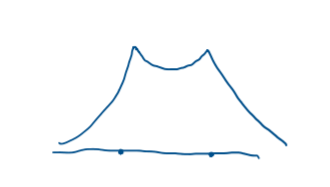
\includegraphics{images/3v1.png}

\textbf{Связывающая орбиталь.} Связывающий характер объясняется интерференцией двух атомных
орбиталей с одинаковыми по знаку амплитудами, что является причиной повышения
амплитуды волновой функции между ядрами. Электрон, занимающий эту орбиталь, с
повышенной вероятностью находится в межъядерном пространстве и может сильнее
взаимодействовать с обоими ядрами. Когда эта орбиталь занята электронами, энергия
молекулы становится ниже, чем энергия изолированных атомов.

$$\psi^* = \psi_A - \psi_B$$
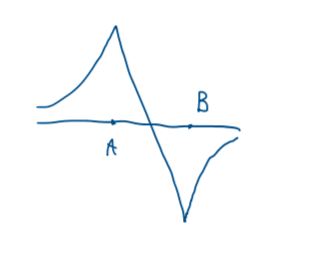
\includegraphics[scale=.750]{images/3v2.png}

\textbf{Разрыхляющая орбиталь.} Большая энергия электрона на этой орбитали возникает
вследствие интерференции двух атомных орбиталей с разными по знаку амплитудами, при
этом амплитуды волновых функций вычитаются и между двумя ядрами образуется узловая
плоскость. Когда эта орбиталь занята электронами, энергия молекулы становится выше,
чем энергия отдельных атомов. Преобладает отталкивание между электронами $\Rightarrow$ 
ослабление связывания атомов. Разрыхляющая орбиталь всегда разрыхляет больше,чем
связывающая - связывает.

Важно, что по ММО для n атомных орбиталей получается n
молекулярных.

Для двухэлектронных систем волновая функция будет равна
произведению одноэлектронных волновых функций. Например,
для молекулы водорода.

$$\psi = \psi_1\cdot\psi_2 = (\psi_A(1)+\psi_B(1))(\psi_A(2)+\psi_B(2))$$

Вероятностное распределение электронной плотности пропорционально квадрату волновой функции:

$$\psi^2 = \psi_A^2 + 2\psi_A\psi_B + \psi_B^2$$
$$\psi^{*2} = \psi_A^2 - 2\psi_A\psi_B + \psi_B^2$$

Интеграл перекрывания:

$$S = \int\psi_a\psi_BdV$$

$$E\pm = \frac{E_F\pm\beta}{q\pm S}$$

$E_A = E_B$ - исходный уровень\\
$\beta$ - резонансный интеграл\\
$S$ - интеграл перекрывания

В области связывания интеграл перекрывания больше нуля, в
области разрыхления меньше нуля. Он также может быть равен
нулю для несвязывающих орбиталей. Чтобы образовалась связь,
должно доминировать положительное перекрывание.

На основании диаграмм молекулярных орбиталей можно
определить магнитные свойства молекулы, общий спин,
кислотность или основность по Льюису, увидеть способные к
донированию или акцептированию орбитали.